\documentclass[a4paper,12pt]{report}

\usepackage{alltt, fancyvrb, url}
\usepackage{graphicx}
\usepackage[utf8]{inputenc}
\usepackage{float}
\usepackage{hyperref}

\hypersetup{
    colorlinks=true,
    linkcolor=black,
    filecolor=magenta,      
    urlcolor=blue,
    pdfpagemode=FullScreen,
    }

\usepackage{titlesec}

\titleformat{\chapter}
  {\Large\bfseries} % format
  {\huge \thechapter} % label
  {20pt}             % sep
  {\huge}           % before-code

\title{Assignment 03 - \\``Smart Temperature Monitoring''\\
    \large ``Embedded Systems e Internet of Things'' final report}

\author{Lorenzo Cinelli}
\date{\today}

\begin{document}

\maketitle

\tableofcontents

\chapter{Analysis}

    \section{Description}
        The required software is a Smart Temperature Monitoring system.\\
        It is made up of a temperature sensor that periodically sends the temperature sampled to a control unit.
        The control unit is in charge of deciding the window opening percentage depending on the temperature -
        in case the window is in \textit{AUTOMATIC MODE}. \\
        If the window is in \textit{MANUAL MODE} it can be controlled manually by an user through the user panel,
        formed by a button to switch the window mode, a potentiometer to manually set the opening of the window,
        and an LCD screen that displays information.\\
        The whole system can be controlled by a dashboard which shows the current values of the system and tracks
        the temperature of the environment.
        The operator by the dashboard is able to restore the system in case of high temperature for prolonged time
        - that sets the system in an alarm state - by pressing a button.
        From the dashboard, it is possible to switch the window mode and also change the opening of the window.\\\\
        \centerline{\href{https://docs.google.com/document/d/1bQZ4LNd35CGHn0wV8lqoz_GF4CWnNGBrRnF0vuKWUDI/edit?usp=sharing}{Here}
        is the complete description of the assignment.}

    \section{Domain Model}

        The system is composed by four subsystems.\\
        The control unit is the back-end of the system in charge of governing and coordinating the whole system.\\
        It establishes the frequency of temperature sampling of the temperature sensor, with whom communicates via
        the mqtt protocol.\\        
        The control unit decides the window opening percentage, based on the temperature,
        if the window is in \textit{AUTOMATIC MODE}.
        It communicates with the window subsystem via serial line. \\\\
        The temperature subsystem has to sample periodically the temperature and send it to the control unit.
        In case of connection problem a red led should be turned on, otherwise in case of conneciton working a green led
        should be turned on.\\\\
        The window subsystem controls the window and has a user panel, from where an user can switch from \textit{AUTOMATIC} to
        \textit{MANUAL} mode and vice versa, can set the opening of the window when it's in \textit{MANUAL MODE} and can see some
        basic information through an lcd display.\\\\
        The dashboard is the front-end of the system and permits to operators to remotely visualize the data and interact
        with the system via the http protocol. \\
        It visualize the current data of the system, including the temperature, the state, the window mode and the window opening.\\
        It also shows a graph representing the temperature history, and highlights the maximum, minimum and average
        temperature measured.
        The other main function of the dashboard is to interact with the system.
        It can manage a temperature alarm and it can switch window mode, setting the opening of the window too.

        \begin{figure}[H]
            \centering{}
            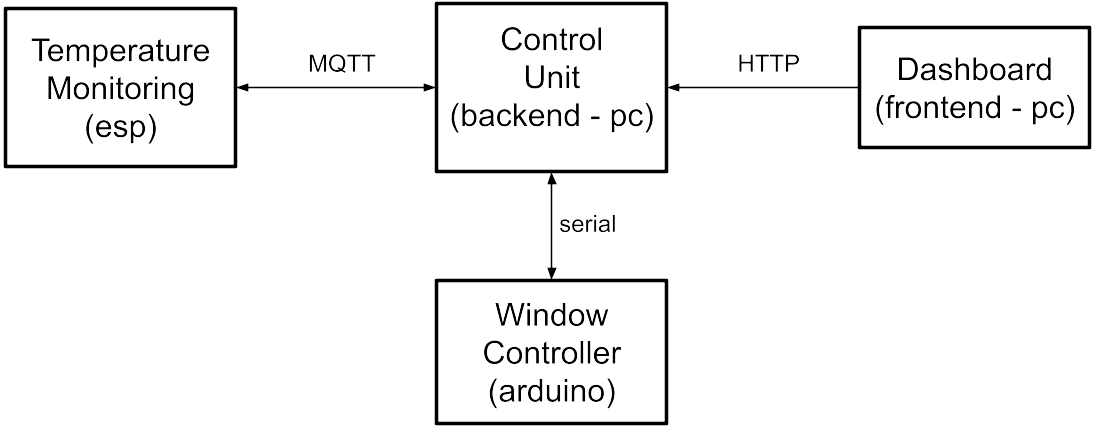
\includegraphics[width=350pt]{report/img/Assignment-03_SMT-Domain.png}
            \caption{Smart Temperature Monitoring}
            \label{img:system}
        \end{figure}


    \section{Requirements}

        \begin{itemize}
            \item The control unit and the temperature sensor have to communicate via the mqtt protocol.
            \item The control unit, the window, and its user panel have to communicate via serial line.
            \item The control unit and the dashboard have to communicate via the http protocol.
            \item The control unit stores the current data of the entire system and tracks the temperature by storing the last
            $N$ measurements, the maximum, the minimum and the average sampled.
            \item The temperature sensor must sample and send to the control unit the temperature at a frequency established by
            the control unit based on the current temperature state (\textit{NORMAL, HOT, TOO\_HOT, ALARM}).
            \item The temperature state is established by the temperature and duration of it.
            \item The window opening is decided by the control unit when the window is in \textit{AUTOMATIC MODE}. It depends by
            the temperature state and the temperature itself.
            \item The window opening when the window is in \textit{MANUAL MODE} is set manually by the user through the user panel,
            or by an operator through the dashboard.
            \item The window mode can be switched by pressing a button in the user panel or in the dashboard.
            \item The dashboard displays the data stored by the control unit, in particular the temperature history is displayed
            in a chart.
            \item When the temperature is too high for too long the system goes in \textit{ALARM} state. To return in
            \textit{NORMAL} state occurs an operator fixing the issue from the dashboard.
        \end{itemize}


        \chapter{Design}

        \section{Architecture}
    
            The system is composed by four modules: the control unit, the temperature monitoring, the window controller and the dashboard. 
            The control unit is the center of the system, able to exchange information between itself and any other module.\\\\
            %
            The temperature monitoring is a task-based architecture with only one task which is a synchronous finite state machine. 
            Despite having only one task produces overhead, it offers great flexibility and modularity.\\\\
            %
            The window controller is a task-based architecture. Tasks are concurrent and are: communication task via serial line, and window 
            controlling task.\\
            Each task interacts with the model that offers encapsulation to physical devices and subsystem data.\\\\
            %
            The dashboard is based on an MVC architectural pattern. The view is formed by two modules: the active GUI and the communication 
            module. \\
            The first one is in charge of displaying updated data in the GUI, while the second submodule periodically sends an HTTP request 
            to the control unit to obtain updated data and eventually send commands.\\\\
            %
            The control unit is an based on an MVC architectural pattern. The view is formed by the communication modules that communicates 
            with the other three subsystem.\\
            The control unit can be seen as the central server of the system, where each one of the communication tasks remains in a 
            listening state ready to process and respond to an incoming message.
    
        \section{Detailed Design}
    
            \paragraph{Temperature Subsystem\\}
                \ \\
                The task in the Temperature Monitoring subsystem deals to send periodically via the MQTT protocol the current temperature of 
                the environment. The period is send via MQTT from the control unit.\\
                The task is described by a \texttt{synchronous finite state machine}. 
    
                \begin{figure}[H]
                    \centering{}
                    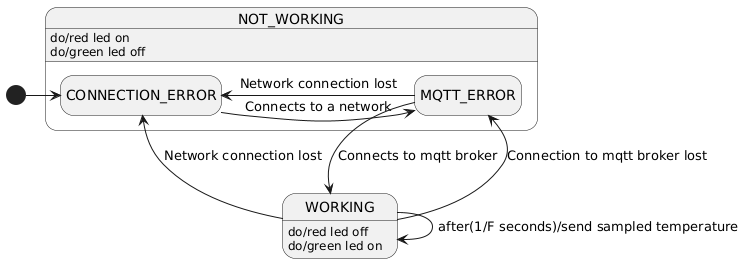
\includegraphics[width=\textwidth]{uml/img/TemperatureCommunicationUML.png}
                    \caption{Temperature Monitoring Connection State}
                    \label{img:connection_state}
                \end{figure}
    
                \begin{itemize}
                    \item NOT\_WORKING: in this state the sensor cannot communicate with the MQTT broker and by consequence with the Control 
                    Unit. To highlight the connection problem a red led is turned on.
                    \item CONNECTION\_ERROR: it's the initial state. It means that the sensor coulden't connect to any network. Each time the 
                    task is executed it will try to connect to the designated network.
                    \item MQTT\_ERROR: in this state the sensor is connected to a network but is not connected to the MQTT broker. Each time 
                    the task is executed it will try to connect to the broker.
                    \item WORKING: the sensor can communicate with the Control Unit. To signal that the connection is working a green led is 
                    turned on. Each time the task is executed the sensor samples the current temperature and send it to the Control Unit. 
                    The Control Unit in response, based on the temperature received, replies with the frequency of temperature sampling.
                \end{itemize}
    
            \newpage
            \paragraph{Window Subsystem\\}
                \ \\
                The Window Controller has two tasks: the communication tasks that sends periodically the subsystem data to the Control Unit 
                and reads any reply from it, and the window task which deals with the window mode, set the opening of the window based on 
                the temperature if in \textit{AUTOMATIC\_MODE} or the percentage set by the user or operator if the window is in 
                \textit{MANUAL\_MODE}.\\
                The window task is described by a \texttt{synchronous finite state machine}.
    
                \begin{figure}[H]
                    \centering{}
                    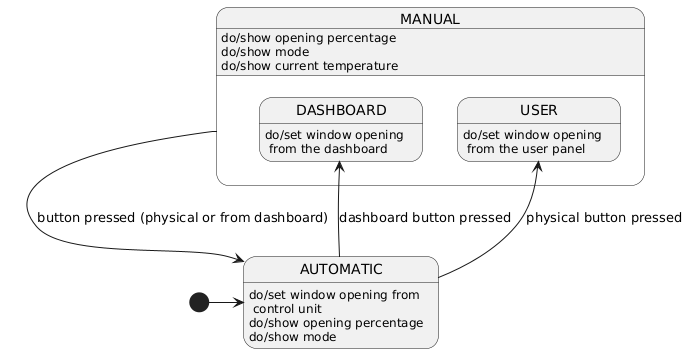
\includegraphics[width=\textwidth]{uml/img/WindowModeUML.png}
                    \caption{Window Mode}
                    \label{img:window_mode}
                \end{figure}
    
                \begin{itemize}
                    \item AUTOMATIC: it's the initial mode of the window. In this mode the opening of the window is established by the 
                    Control Unit depending on the current temperature state and temperature. 
                    \item MANUAL: in this mode the window opening is established by an user or an operator, depending on where the command 
                    came from.
                    \item USER: in this mode is an user who sets the opening of the window by the provided user panel.
                    \item DASHBOARD: in this mode is an operator who sets the opening of the window by the dashboard.
                \end{itemize}
    
            \newpage
            \paragraph{Control Unit Subsystem\\}
                \ \\
                The Control Unit is designed to store the data of the system, compute the frequency of temperature sampling and the opening 
                of the window, as well as manage communication between itself and the rest of the system.\\
                The frequency of sampling and the opening of the window are calculated by the temperature state, determined by the current 
                temperature.\\
                The temperature task is described by a \texttt{synchronous finite state machine}. 
    
                \begin{figure}[H]
                    \centering{}
                    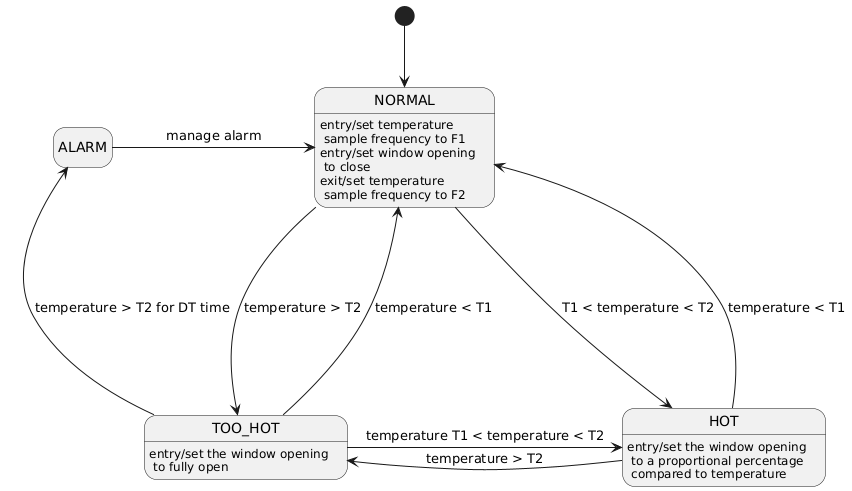
\includegraphics[width=\textwidth]{uml/img/TemperatureStateUML.png}
                    \caption{Temperature State}
                    \label{img:temperature_state}
                \end{figure}
    
                \begin{itemize}
                    \item NORMAL: it's the initial state. In this state the temperature is normal, so the window is closed.
                    \item HOT: in this state the temperature begins to be hot, so depending on the current temperature the window will be 
                    opened for a certain percentage.
                    \item TOO\_HOT: in this state the environmental temperature is too hot. The window must be fully open.
                    \item ALARM: if the temperature state remains in \textit{TOO\_HOT} for $DT$ time then the system goes in \textit{ALARM} 
                    state. In this state the window is fully open until an operator manually manages the alarm from the dashboard.
                \end{itemize}

    
\end{document}
